\subsubsection{Analisis Operasi Write}
\label{subsubsection:analisis-operasi-write}

Analisis kinerja operasi \textit{write} merupakan inti dari penilitian ini, seperti yang sudah dijelaskan pada Bagian \ref{sec:rumusan-masalah}. Analisis ini bertujuan untuk memvalidasi bahwa \textit{erasure coding} dapat mengungguli replikasi dalam kondisi tertentu. Analisis kinerja operasi \textit{write} akan dibagi berdasarkan skenario yang sudah disebutkan pada Bagian \ref{subsubsection:setup-benchmark}. Setiap skenario akan dianalisis berdasarkan hasil \textit{benchmark} yang telah dilakukan.

\begin{enumerate}
  \item Skenario 1: Internet cepat dan \textit{payload} kecil

  Pada skenario pertama yang dirancang sebagai kondisi ekstrem yang menguntungkan replikasi, hasil \textit{benchmark} menunjukkan bahwa sistem replikasi memiliki \textit{response time} yang lebih rendah dibandingkan sistem berbasis \textit{erasure coding}. Perbedaan kinerja ini dapat dilihat pada Gambar \ref{fig:write-smload-fastnet}.

  \begin{figure}[ht]
      \centering
      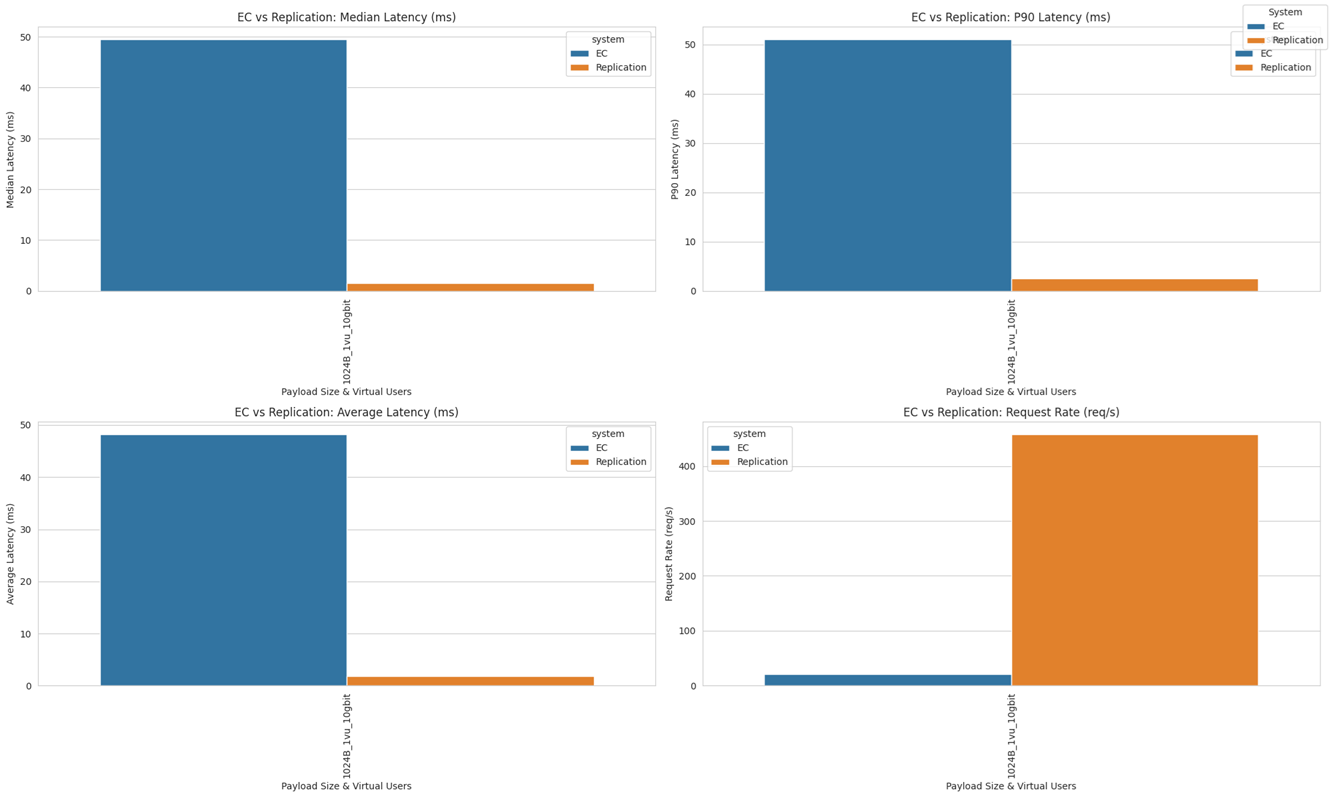
\includegraphics[width=0.8\textwidth]{resources/chapter-4/write_smload_fastnet.png}

      \caption{Kinerja Operasi Write pada Internet Cepat dan Payload Kecil}
      \label{fig:write-smload-fastnet}
  \end{figure}

  Interpretasi dari hasil ini terletak pada dinamika komponen latensi. Pada jaringan dengan \textit{bandwidth} tinggi seperti 10 Gbps, waktu yang dibutuhkan untuk mentransfer data menjadi kecil. Selain itu, data yang kecil membuat operasi terkait data seperti penulisan pada \textit{memory} dan \textit{disk} menjadi kecil juga. Dengan kecilnya waktu transfer dan operasi terkait data, faktor penentu \textit{response time} adalah biaya komputasi dan \textit{overhead} pemrosesan pada setiap node. Hal ini dibuktikan dengan hasil \textit{trace} pada setiap operasi eksternal dari \textit{node} yang memiliki waktu hampir sama baik untuk replikasi dan juga \textit{erasure coding}. Sisa waktu yang tidak terdapat pada grafik ini berarti merupakan waktu yang diperlukan untuk proses konsensus dan juga \textit{erasure coding}. Hasil \textit{trace} dapat dilihat pada Gambar \ref{fig:write-smload-fastnet-trace}.

  Dalam skenario ini, proses \textit{erasure coding} yang lebih kompleks membutuhkan waktu yang lebih lama dibandingkan dengan proses replikasi yang lebih sederhana. Lingkungan seperti ini umum ditemukan pada komunikasi antar-\textit{server} dalam satu pusat data modern dengan penggunaan transaksi data berukuran kecil seperti pembaruan metadata, status sesi, atau operasi konfigurasi singkat.

  \begin{figure}[ht]
    \centering
    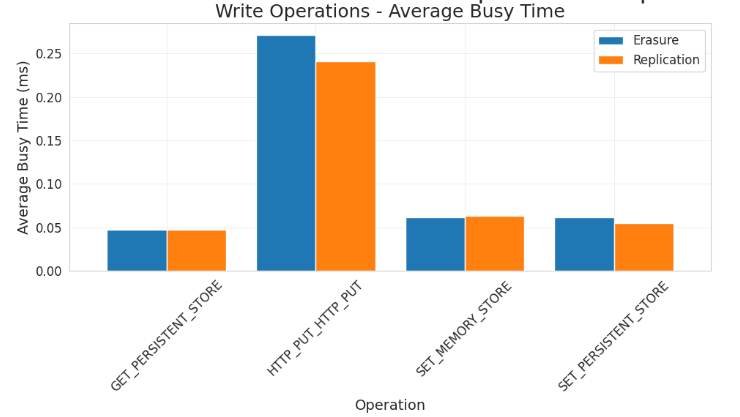
\includegraphics[width=0.8\textwidth]{resources/chapter-4/write_smload_fastnet_trace.png}

    \caption{Trace Operasi pada Internet Cepat dan Payload Kecil}
    \label{fig:write-smload-fastnet-trace}
  \end{figure}
  
  \item Skenario 2: Internet lambat dan \textit{payload} besar
  
  Skenario kedua dirancang sebagai kondisi ekstrem yang berlawanan dengan skenario pertama dengan keuntungan pada \textit{erasure coding}. Hasil \textit{benchmark} pada skenario ini menunjukkan pembalikan kinerja dramatis dengan sistem berbasis \textit{erasure coding} secara konsisten mengungguli replikasi dengan \textit{response time} yang lebih rendah untuk \textit{payload} yang diuji. Gambar \ref{fig:write-bigload-slownet} menunjukkan perbandingan kinerja operasi \textit{write} pada skenario ini.

  \begin{figure}[ht]
      \centering
      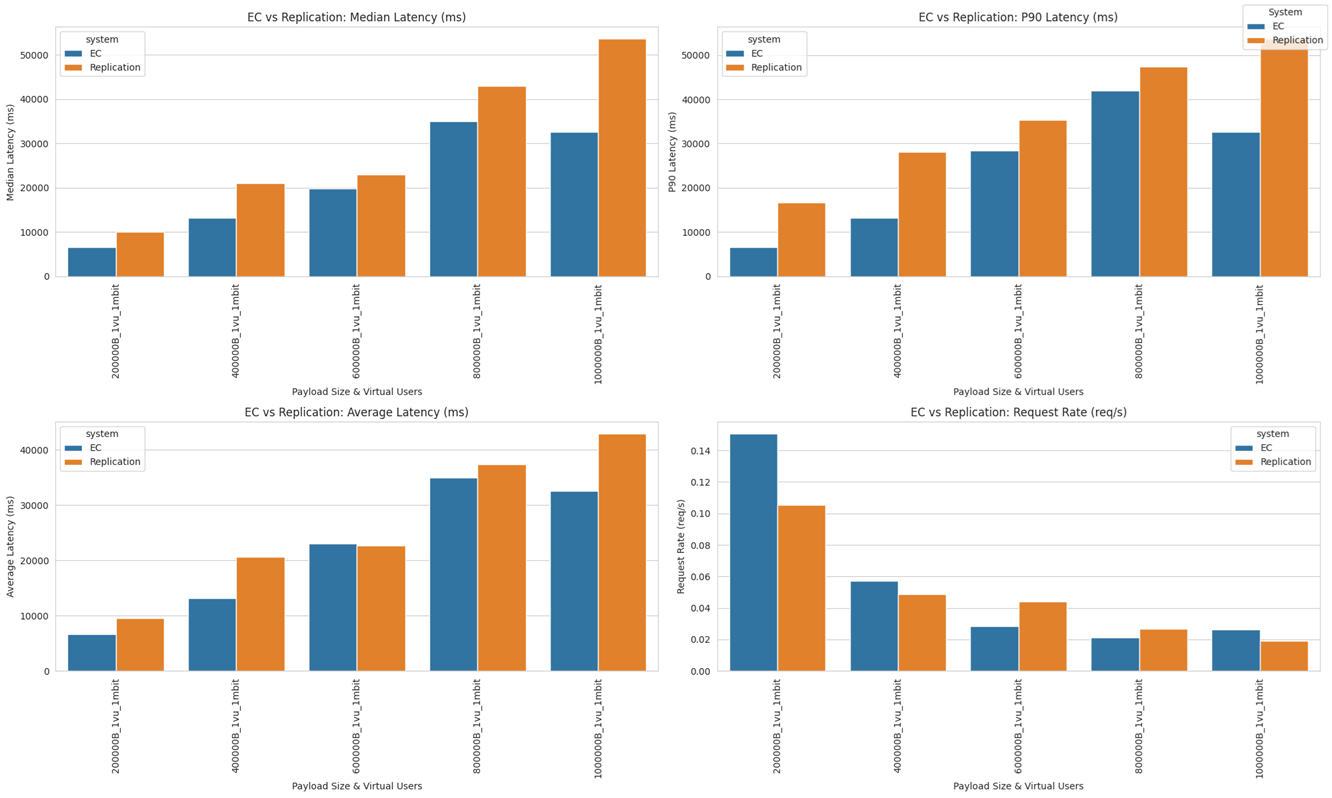
\includegraphics[width=0.8\textwidth]{resources/chapter-4/write_bigload_slownet.png}

      \caption{Kinerja Write pada Internet Lambat dan Payload Besar}
      \label{fig:write-bigload-slownet}
  \end{figure}

  Hasil dari skenario ini mengkonfirmasi bahwa \textit{erasure coding} dapat mengungguli replikasi dalam kondisi tertentu, yaitu dalam skenario dengan \textit{bandwidth} rendah dan untuk \textit{payload} yang besar. Dalam kondisi ini, waktu transfer data menjadi faktor dominan dalam \textit{response time}. Proses \textit{erasure coding} walaupun lebih kompleks, dapat memberikan \textit{latensi} lebih cepat karena mengurangi jumlah data yang harus ditransfer serta dioperasikan. Lingkungan seperti ini umum ditemukan pada aplikasi yang beroperasi dengan sumber daya jaringan terbatas, seperti aplikasi \textit{internet of things} yang tersebar di area luas, \textit{edge computing}, atau pencadangan data melalui koneksi internet yang lambat. Hal ini dibuktikan dengan hasil \textit{trace} yang menunjukkan peningkatan signifikan dari waktu \textit{set} untuk replikasi pada \textit{persistent store}. Hasil \textit{trace} dapat dilihat pada Gambar \ref{fig:write-bigload-slownet-trace}.

  \begin{figure}[ht]
      \centering
      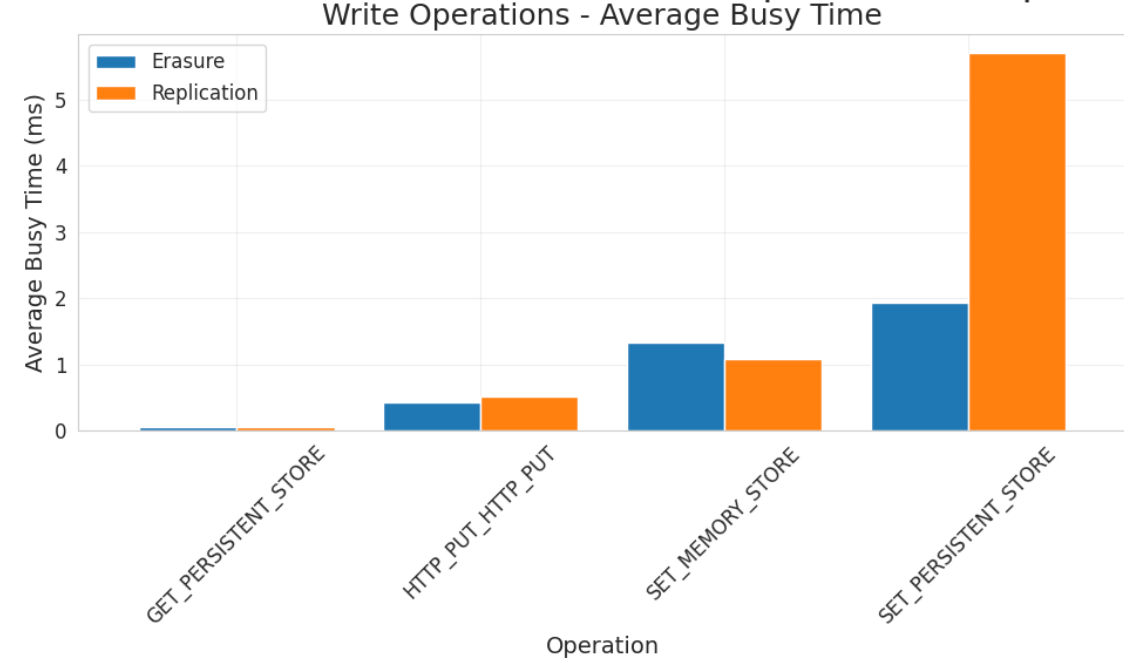
\includegraphics[width=0.8\textwidth]{resources/chapter-4/write_bigload_slownet_trace.png}

      \caption{Trace Operasi pada Internet Lambat dan Payload Besar}
      \label{fig:write-bigload-slownet-trace}
  \end{figure}

  \item Skenario 3: Internet menengah dan \textit{payload} besar
  
  Dengan didapatkannya bahwa \textit{erasure coding} dapat mengungguli replikasi pada skenario kedua, skenario ketiga dirancang untuk mengeksplorasi titik perbatasan ketika keunggulan kinerja beralih dari sistem \textit{erasure coding} ke sistem replikasi. Seperti yang sudah dijelaskan pada Bagian \ref{subsubsection:setup-benchmark}, skenario ini dirancang dengan merepresentasikan kondisi jaringan dengan \textit{bandwidth} rata-rata internet di Indonesia pada saat penulisan, yaitu 40 Mbps, dengan penambahan atau pengurangan linear.
  
  \begin{figure}[ht]
    \centering
    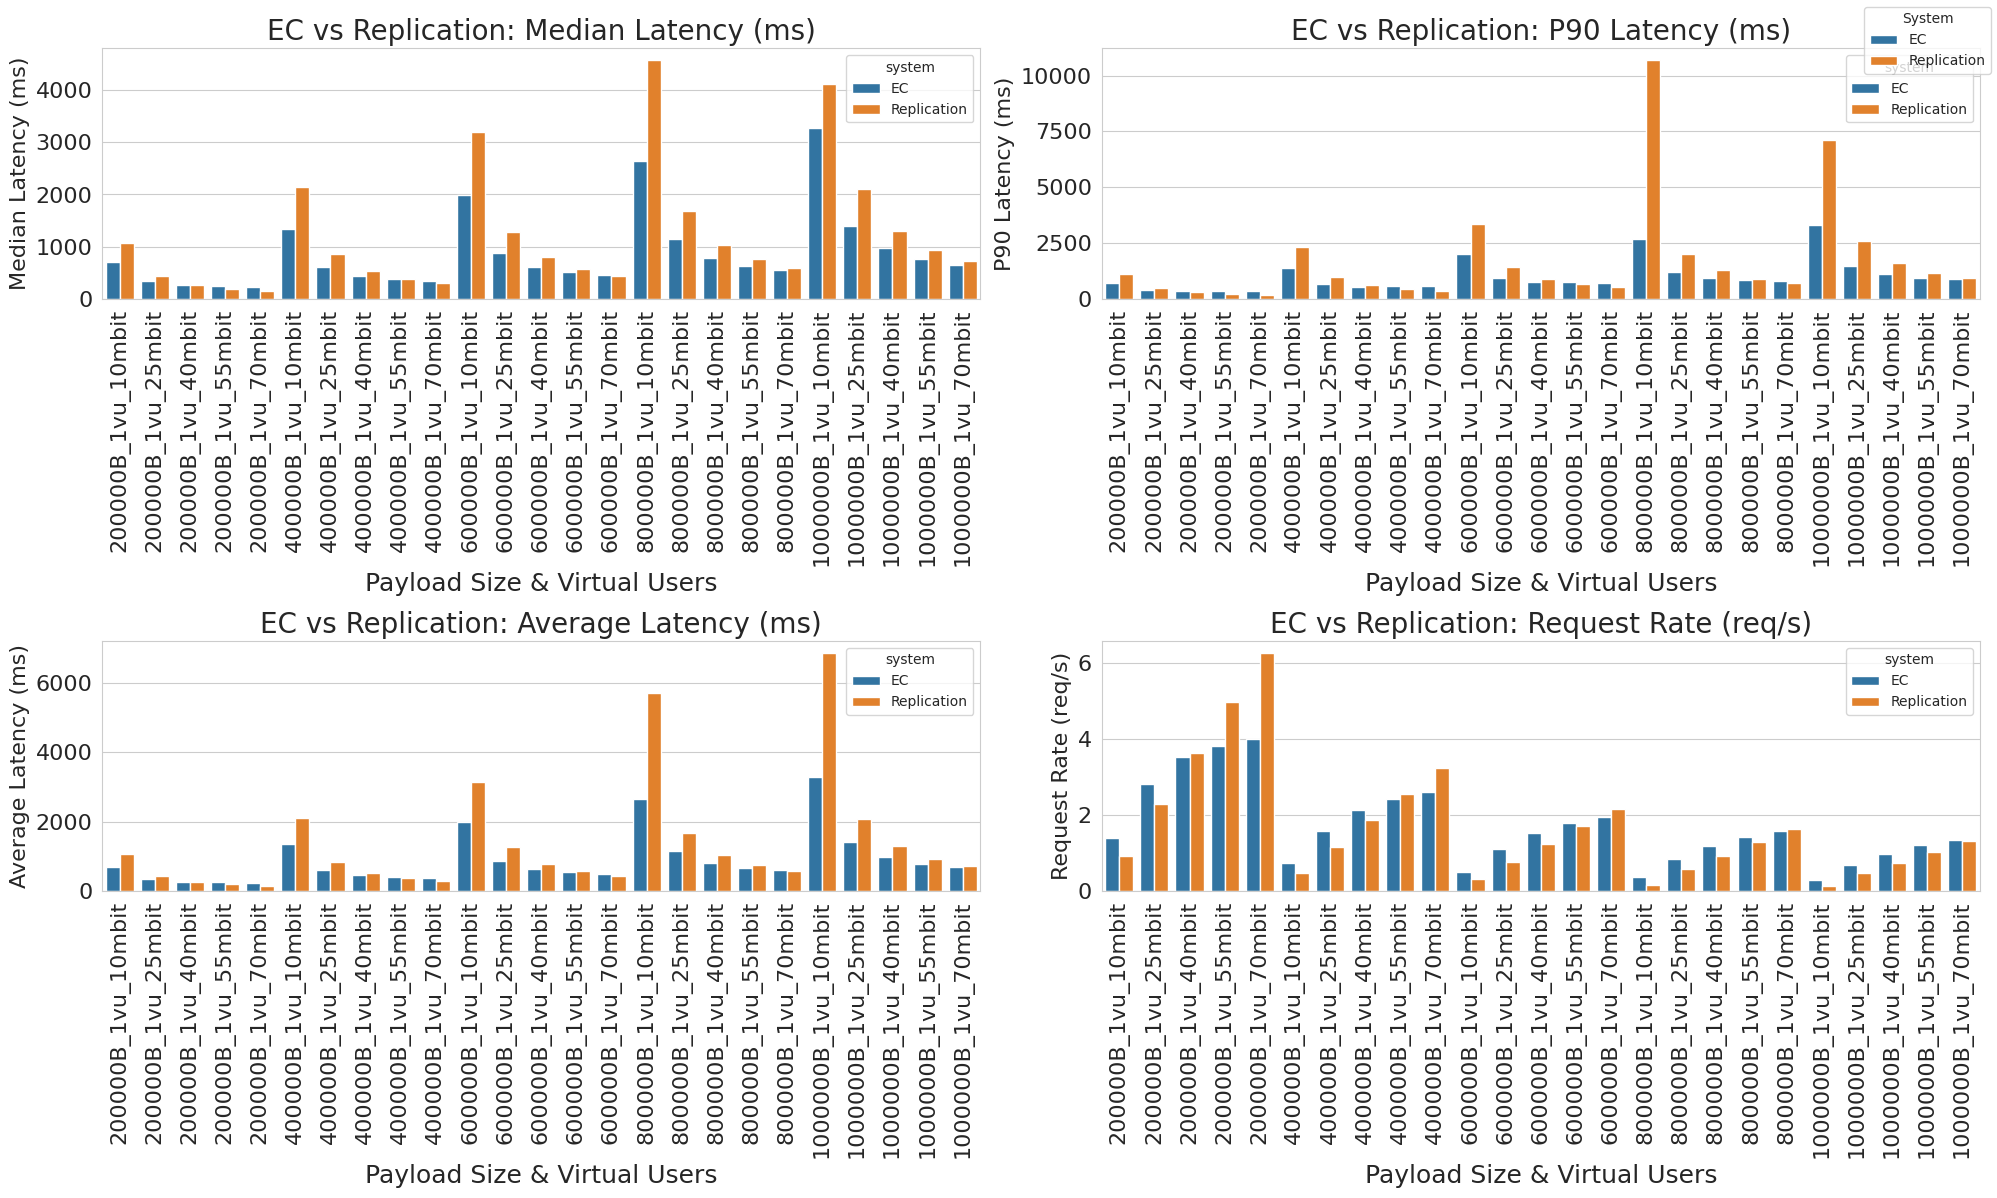
\includegraphics[width=0.8\textwidth]{resources/chapter-4/write_bigload_avgnet.png}

    \caption{Kinerja Write pada Internet Menengah dan Payload Besar}
    \label{fig:write-bigload-avgnet}
  \end{figure}

  Skenario ini menggunakan kombinasi \textit{payload} dan \textit{bandwidth} yang beragam sehingga memberikan diagram dengan grafik yang lebih kompleks. Gambar \ref{fig:write-bigload-avgnet} menunjukkan hasil \textit{benchmark} untuk skenario ini. Dari grafik tersebut, terlihat bahwa keunggulan \textit{erasure coding} semakin berkurang seiring dengan peningkatan \textit{bandwidth} dan penurunan ukuran \textit{payload}. Pada titik tertentu, sistem berbasis replikasi mulai mengungguli sistem berbasis \textit{erasure coding}. Titik impas terjadi ketika penghematan waktu dari transfer data yang lebih sedikit pada \textit{erasure coding} setara dengan penambahan waktu dari proses komputasi \textit{encoding}.

  Untuk memudahkan visualisasi, Gambar \ref{fig:write-bigload-avgnet-heatmap} menunjukkan rasio kinerja dari hasil \textit{benchmark} terhadap \textit{payload} dan \textit{bandwidth} yang digunakan dalam persen. Warna biru dan nilai negatif menunjukkan keunggulan sistem berbasis \textit{erasure coding}, sedangkan warna merah dan nilai positif menunjukkan keunggulan sistem berbasis replikasi. Titik impas terlihat pada area transisi antara warna biru dan merah.  Kode yang digunakan untuk menghasilkan gambar ini dapat dilihat pada repository Github hasil implementasi. Terdapat anomali yang terjadi ketika \textit{payload} terlalu besar dan \textit{bandwidth} terlalu rendah, hal ini disebabkan oleh \textit{timeout} dan kegagalan jaringan yang terjadi pada antarmuka \textit{client}.

  \begin{figure}[ht]
    \centering
    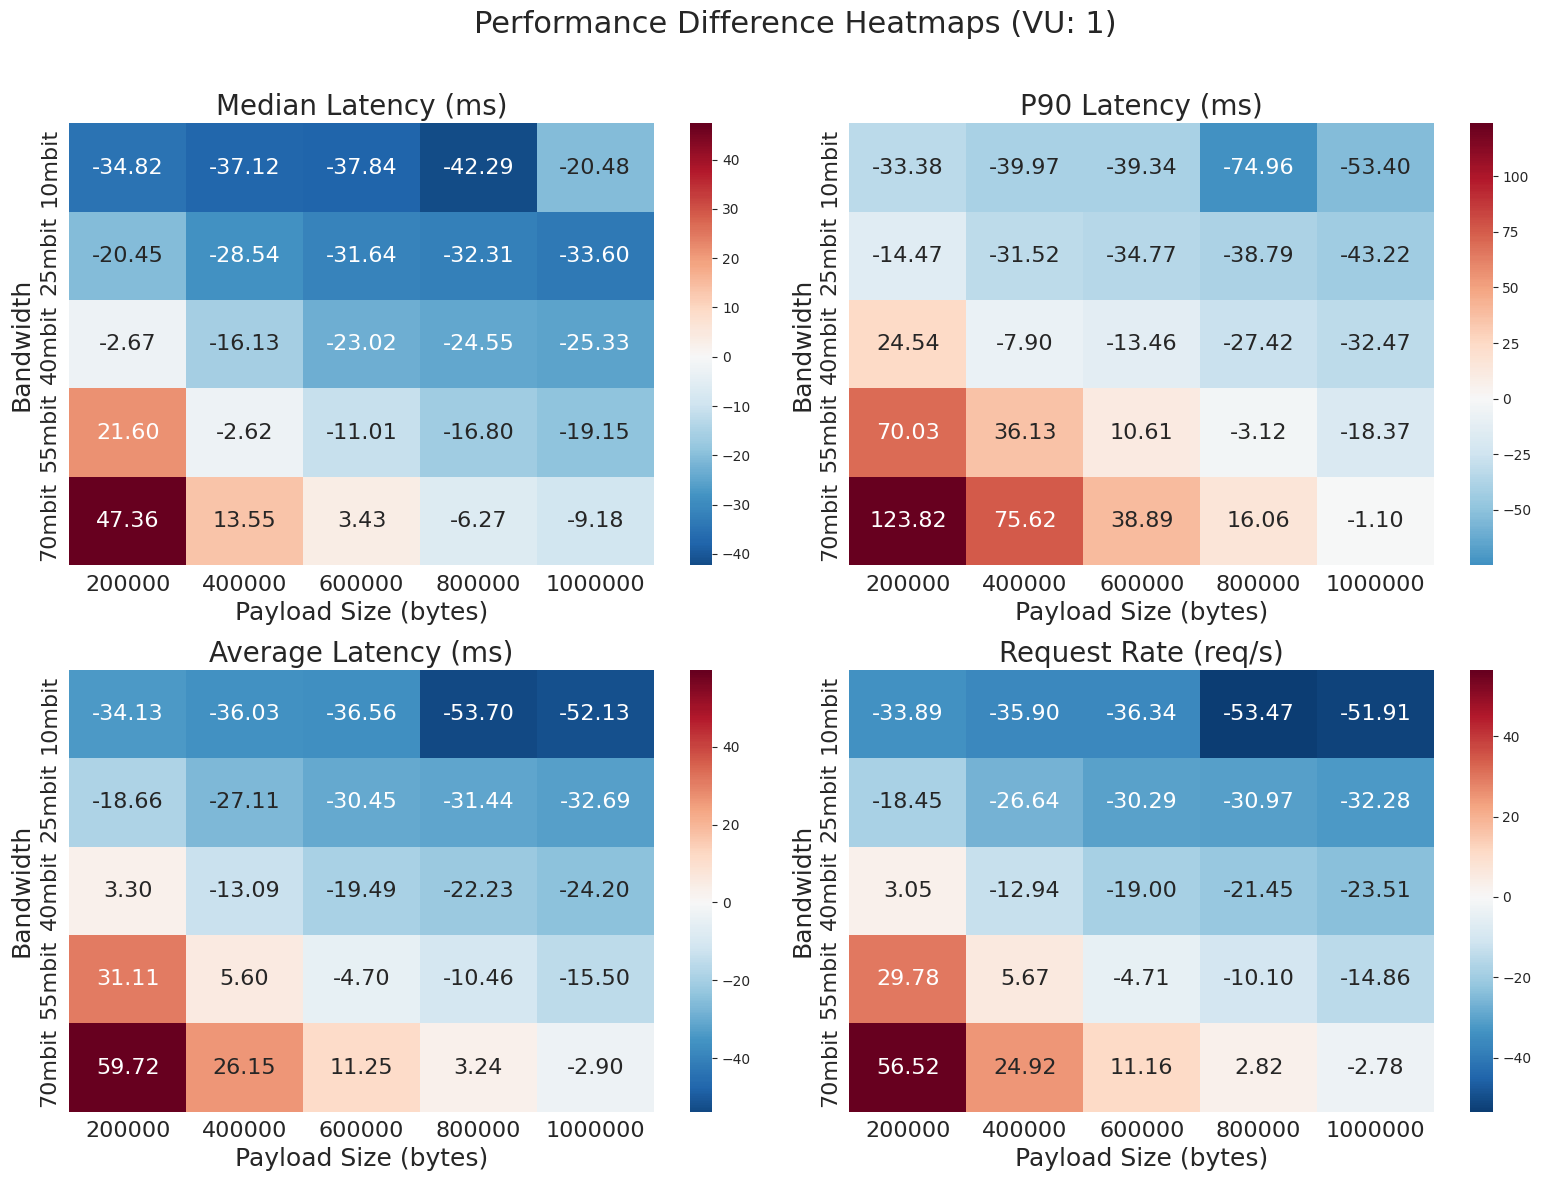
\includegraphics[width=0.8\textwidth]{resources/chapter-4/write_bigload_avgnet_heatmap.png}

    \caption{Heatmap Write pada Internet Menengah dan Payload Besar}
    \label{fig:write-bigload-avgnet-heatmap}
  \end{figure}

  Untuk menggambarkan perolehan titik impas, dapat dibuat diagram garis yang menunjukkan rata-rata \textit{response time} sistem berbasis \textit{erasure coding} dan replikasi terhadap \textit{bandwidth} dan ukuran \textit{payload}. Gambar \ref{fig:write-bigload-avgnet-line} menunjukkan diagram garis tersebut.

  \begin{figure}[!htbp]
    \centering
    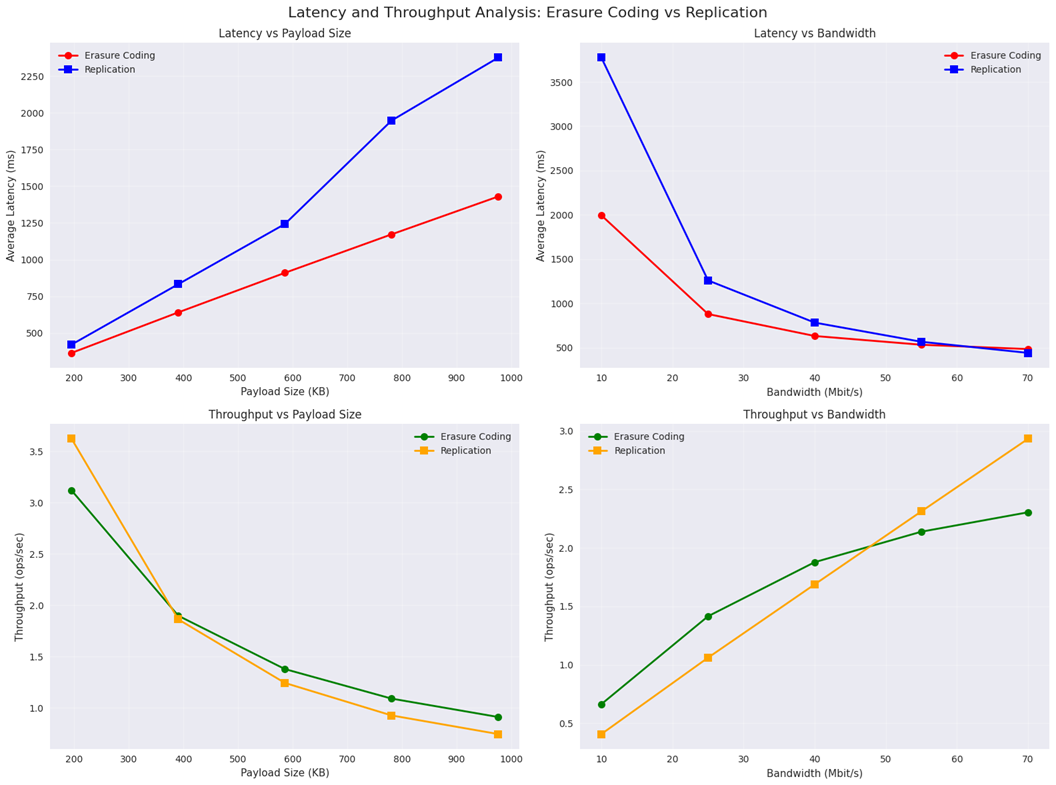
\includegraphics[width=0.8\textwidth]{resources/chapter-4/write_bigload_avgnet_line.png}

    \caption{Diagram Garis Write pada Internet Menengah dan Payload Besar}
    \label{fig:write-bigload-avgnet-line}
  \end{figure}
  
  Namun, untuk mendapatkan nilai yang tepat untuk titik impas antara sistem berbasis \textit{erasure coding} dan sistem berbasis replikasi, perlu dilakukan analisis lebih lanjut. Analisis untuk mendapatkan titik impas dilakukan secara menurunkan hasil \textit{benchmark} yang sudah dilakukan menjadi fungsi menggunakan pendekatan regresi. Fungsi ini kemudian digunakan untuk memperkirakan titik impas. Sebelum melakukan regresi, perlu dilihat \textit{scatter plot} dari hasil \textit{benchmark} sebagai gambaran visual relasi antara \textit{bandwidth}, ukuran \textit{payload}, dan \textit{response time}. Gambar \ref{fig:write-bigload-avgnet-scatter} menunjukkan \textit{scatter plot} tersebut.

  \begin{figure}[ht]
    \centering
    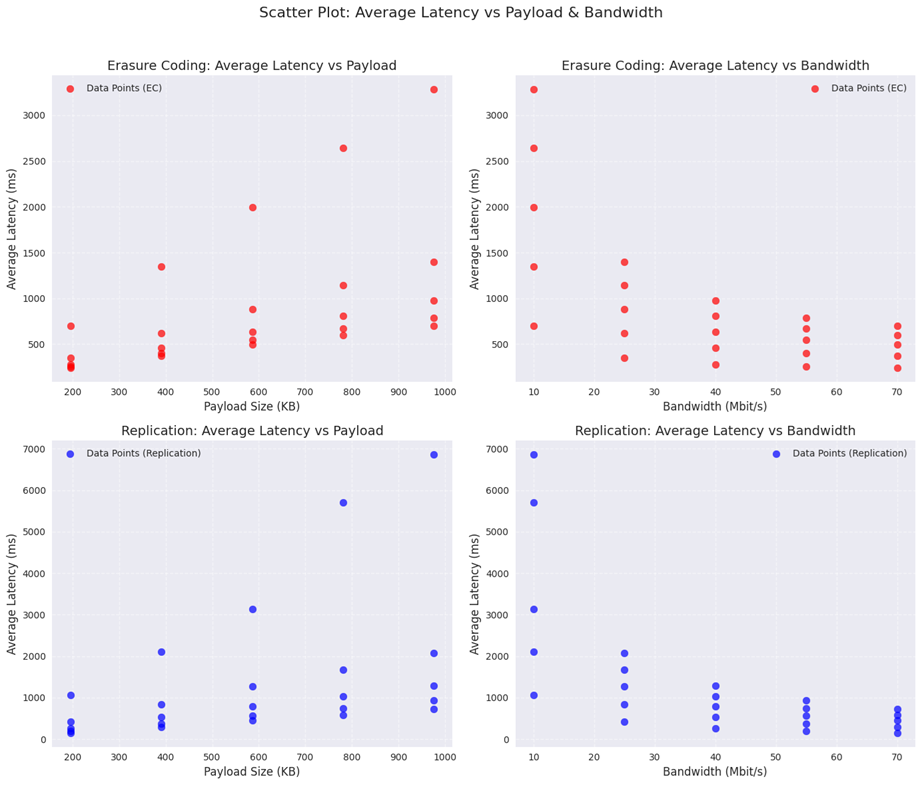
\includegraphics[width=0.8\textwidth]{resources/chapter-4/write_bigload_avgnet_scatterplot.png}

    \caption{Scatter Plot Write pada Internet Menengah dan Payload Besar}
    \label{fig:write-bigload-avgnet-scatter}
  \end{figure}

  Dari \textit{scatter plot} tersebut, terlihat bahwa hubungan dari \textit{bandwidth} dan ukuran \textit{payload} terhadap \textit{response time} tidak linear. Data yang dimiliki hanya sedikit, yaitu 25 data, sehingga regresi yang dilakukan harus mempertimbangkan risiko \textit{overfitting} yang tinggi. Selain itu, disebabkan lingkungan eksperimen dilakukan pada komputer pribadi, \textit{noise} dari eksperimen dapat mempengaruhi hasil. Dengan mempertimbangkan semua hal tersebut, regresi dilakukan dengan model \textit{ridge regression}. Model ini dipilih karena dapat menangani data yang memiliki banyak \textit{noise} serta mengurangi risiko \textit{overfitting} dengan menambahkan bias pada model regresi.

  Model \textit{ridge regression} gabungan dari \textit{bandwidth} dan \textit{payload} terhadap \textit{response time} menghasilkan model tiga dimensi seperti yang ditunjukkan pada Gambar \ref{fig:write-bigload-avgnet-regression}.

  \begin{figure}[ht]
    \centering
    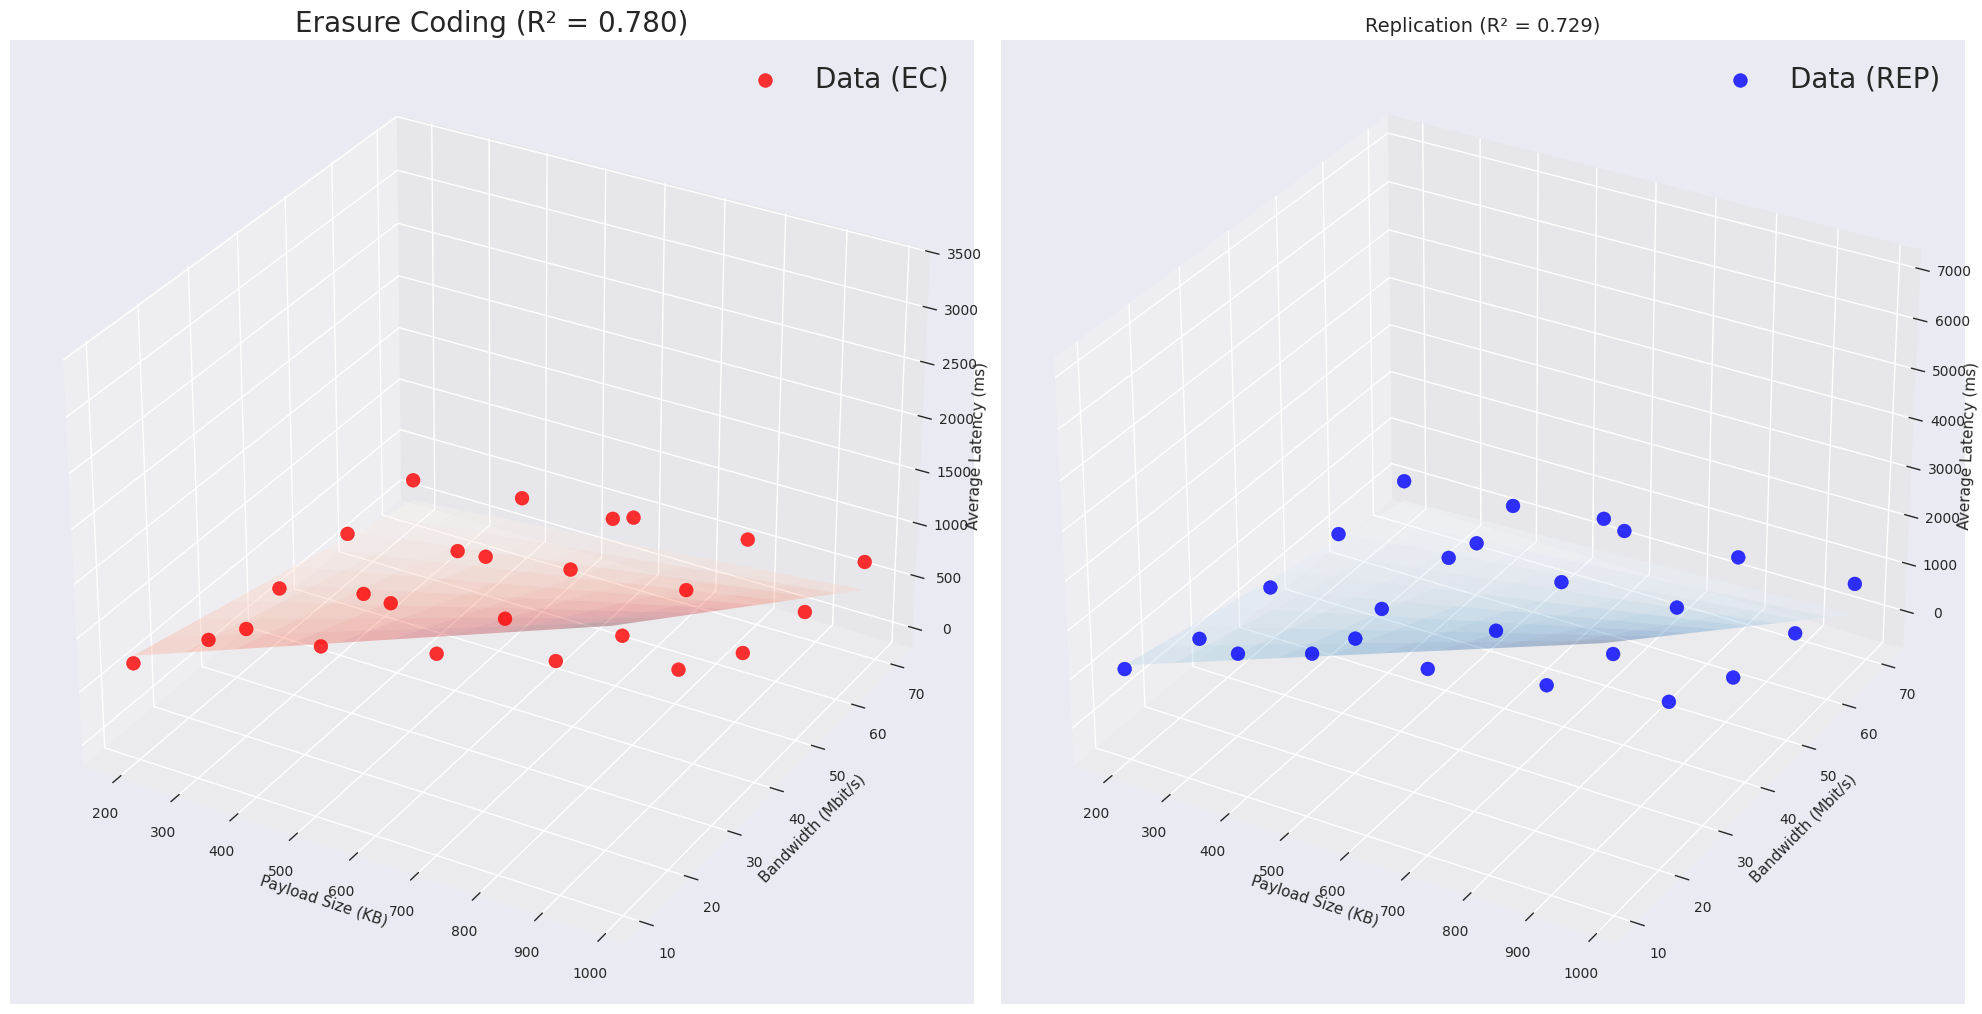
\includegraphics[width=0.8\textwidth]{resources/chapter-4/write_bigload_avgnet_regression.png}

    \caption{Model Regresi Operasi Write}
    \label{fig:write-bigload-avgnet-regression}
  \end{figure}

  Dari model regresi yang dilakukan, kurva pendekatan titik impas antara sistem berbasis \textit{erasure coding} dan sistem berbasis replikasi dapat dihasilkan dengan mencari perpotongan dari model regresi tersebut. Perpotongan didapat dengan menggunakan selisih dan selisih bernilai nol merupakan titik impas. Gambar \ref{fig:write-bigload-avgnet-boundary} menunjukkan analisis titik impas yang dilakukan dengan menggunakan model regresi. Dari perpotongan tersebut dapat dimodelkan menjadi persamaan kurva matematis yang dapat digunakan untuk memperkirakan titik impas pada \textit{bandwidth} dan ukuran \textit{payload} tertentu dengan nilai di atas kurva berarti sistem berbasis \textit{erasure coding} mengungguli sistem berbasis replikasi, dan nilai di bawah kurva berarti sebaliknya.


  \begin{figure}[ht]
    \centering
    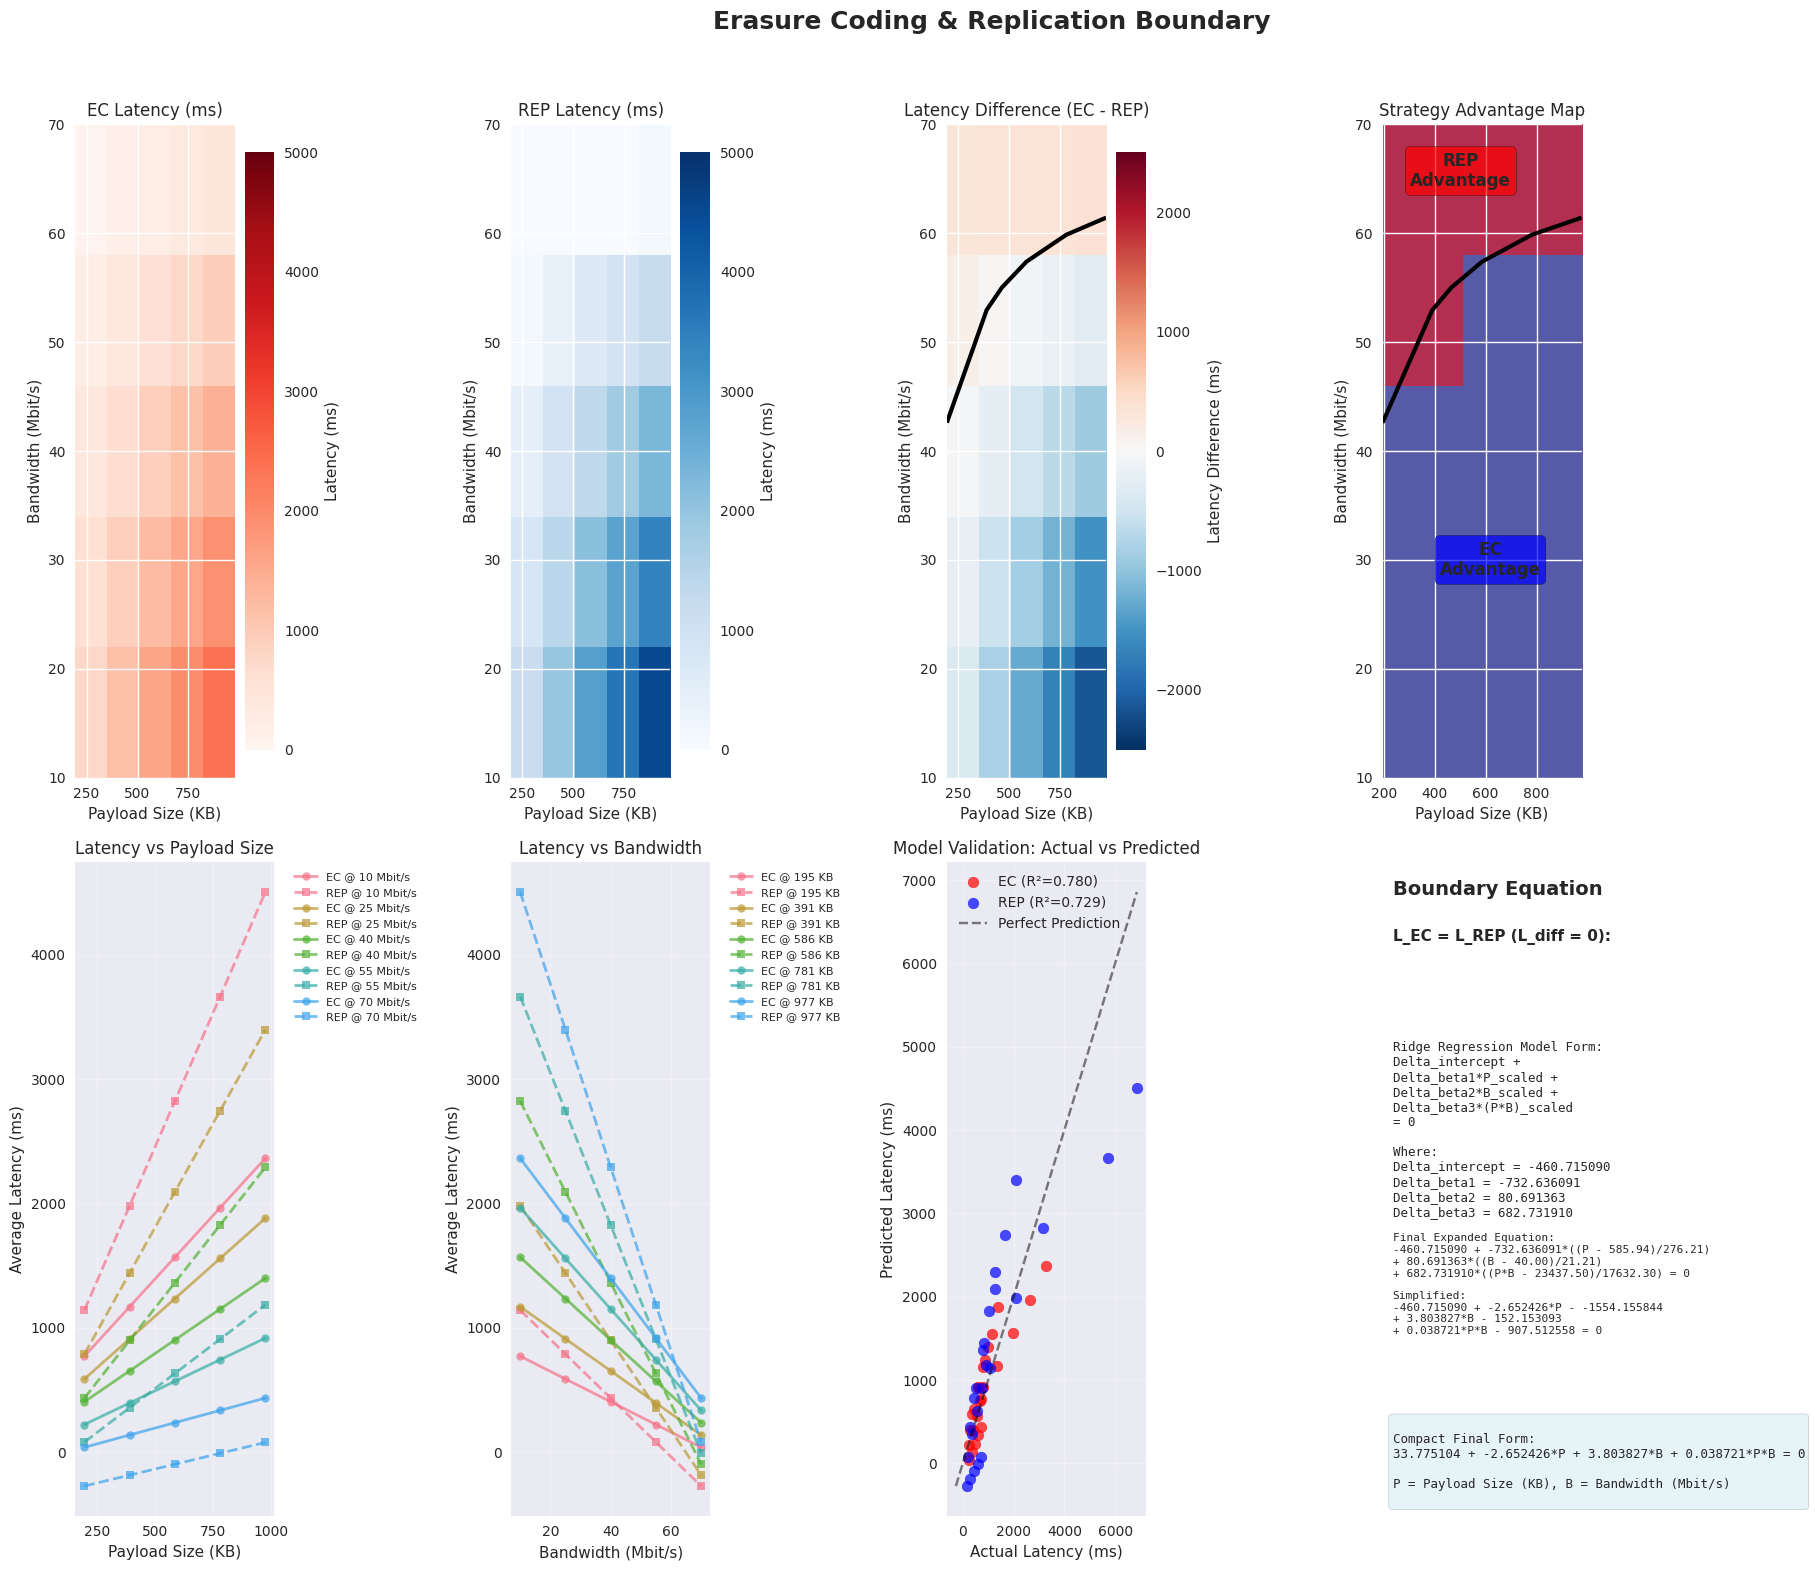
\includegraphics[width=\textwidth]{resources/chapter-4/write_bigload_avgnet_boundary.png}

    \caption{Analisis Titik Impas pada Operasi Write}
    \label{fig:write-bigload-avgnet-boundary}
  \end{figure}

  Kode yang digunakan untuk melakukan regresi ini dapat dilihat pada repository Github hasil implementasi. Perlu diketahui juga bahwa model regresi ini tidak mempertimbangkan faktor lain seperti kecepatan komputasi dari sistem yang digunakan, kecepatan akses memori, kecepatan akses disk, ataupun faktor lain yang dapat mempengaruhi \textit{response time}. Model ini hanya valid pada kondisi dan lingkungan eksperimen yang dilakukan.

\end{enumerate}